\documentclass[conference]{IEEEtran}
% Add the compsoc option for Computer Society conferences.
%
% If IEEEtran.cls has not been installed into the LaTeX system files,
% manually specify the path to it like:
% \documentclass[conference]{../sty/IEEEtran}





% Some very useful LaTeX packages include:
% (uncomment the ones you want to load)



\ifCLASSINFOpdf
  \usepackage[pdftex]{graphicx}
  % declare the path(s) where your graphic files are
  % \graphicspath{{../pdf/}{../jpeg/}}
  % and their extensions so you won't have to specify these with
  % every instance of \includegraphics
  % \DeclareGraphicsExtensions{.pdf,.jpeg,.png}




%\hyphenation{op-tical net-works semi-conduc-tor}
\usepackage{authblk}

\begin{document}
%
% paper title
% can use linebreaks \\ within to get better formatting as desired
\title{Voronoi Diagrams - An exhaustive study with applications.}


% author names and affiliations
% use a multiple column layout for up to three different
% affiliations

%\author[1]{Mrs. Shantha Rangaswamy\thanks{shantharangaswamy@rvce.edu.in}}
%\author[2]{Dr. Shobha G\thanks{shobhag@rvce.edu.in}}
%\author[3]{Dr.B.L.Shivakumar\thanks{shivakumarbl@rvce.edu.in}}
%\author[4]{Samir Sheriff\thanks{samiriff@gmail.com}}
%\author[5]{Satvik N\thanks{nsatvik@gmail.com}}
%
%\affil[1]{shantharangaswamy@rvce.edu.in, Assistant Professor, Department of Computer Science, RV College of Engineering.}
%\affil[2]{shobhag@rvce.edu.in, Dean PG Studies (CSE and ISE), Department of Computer Science, RV College of Engineering.}
%\affil[3]{shivakumarbl@rvce.edu.in, HOD, Department of Civil Engineering, RV College of Engineering.}
%\affil[4]{samiriff@gmail.com, 7th semester BE, Department of Computer Science, RV College of Engineering.}
%\affil[5]{nsatvik@gmail.com, 7th semester BE, Department of Computer Science, RV College of Engineering.}


%\author{
%\IEEEauthorblockN{Dr. N. K. Cauvery}
%\IEEEauthorblockA{Professor\\ Department of Computer Science\\RV College of Engineering\\
%Email: cauverynk@rvce.edu.in}
%\and
%\IEEEauthorblockN{Sandhya S}
%\IEEEauthorblockA{Assistant Professor\\ Department of Computer Science\\RV College of Engineering\\
%Email:sandhya.sampangi@rvce.edu.in}
%\and 
%\IEEEauthorblockN{Satvik N}
%\IEEEauthorblockA{BE 7 semester\\ Department of Computer Science\\RV College of Engineering\\
%Email:nsatvik@gmail.com}
%\and
%\IEEEauthorblockN{Vaishakh BN}
%\IEEEauthorblockA{BE 7 semester\\ Department of Computer Science\\RV College of Engineering\\
%Email: vaishakhbn@gmail.com}
%
%}
\author{
    Samir Sheriff\\
	Student 8th Semester\\
	Department of Computer Science\\
	RV College of Engineering\\
	Email : samiriff@gmail.com
  \and
	Vinay BS.\\
	Student 8th Semester\\
	Department of Computer Science\\
	RV College of Engineering\\
	Email : bsv0099@gmail.com
    \and
    Satvik N\\
    Student 8 semester\\
	Department of Computer Science\\
	RV College of Engineering\\
    Email : nsatvik@gmail.com
}



% make the title area
\maketitle


\begin{abstract}
%\boldmath
A Voronoi diagram is a decomposition of a given space, determined by distances to a specified family of
objects (subsets) in space. These objects are usually called the sites or the generators and to each such object, one associates a corresponding
Voronoi cell, namely the set of all points in the given space whose distance to the given object is not greater than their distance to the other objects. Voronoi diagrams can be found in a large number of fields in science and technology, even in art, and they have found numerous practical and theoretical
applications. It is the technique that enables the division of such multi-dimensional spaces into
subspaces.



This paper deals with an exhaustive study of Voronoi Diagrams, different algorithms pertaining to it and
its real-world applications, which will be explained with the aid of multimedia technology.

\end{abstract}
\begin{keywords}
decision tree, machine learning, genetic algorithms, decision problems.
\end{keywords}

\IEEEpeerreviewmaketitle



\section{Introduction}
Voronoi diagram is a decomposition of a given space, determined by distances to a
specied family of objects (subsets) in the space. These objects are usually called
the sites or the generators and to each such object one associates a corresponding
Voronoi cell, namely the set of all points in the given space whose distance to the
given object is not greater than their distance to the other objects. It is named after
Georgy Voronoi, and is also called a Voronoi tessellation, a Voronoi decomposition,
or a Dirichlet tessellation (after Lejeune Dirichlet). Voronoi diagrams can be found
in a large number of elds in science and technology, even in art, and they have
found numerous practical and theoretical applications. It is the technique that
enables the division of such multi-dimensional spaces into subspaces.


\section{Introduction to Voronoi Digrams}
\subsection{Decision Trees}

\begin{itemize}
\item{\textbf{ID3} (Iterative Dichotomiser 3)}
\item{\textbf{C4.5} algorithm, successor of ID3}
\item{\textbf{CART} (Classification And Regression Tree)}
\item{\textbf{CHi-squared Automatic Interaction Detector }(CHAID). Performs multi-level splits when computing classification trees.}
\item{\textbf{MARS}: extends decision trees to better handle numerical data}
\end{itemize}



\subsection{Genetic Algorithms}


A GA generally has four components. 


The following is a typical GA procedure:

\begin{itemize}
\item{Create an initial population of random genomes.}
\item{Loop through the genetic algorithm, which produces a new generation every iteration.}

\begin{itemize}
\item{Assess the fitness of each genome, stopping if a solution is found.}
\item{Evolve the next generation through natural selection and reproduction.}

\begin{itemize}
\item{Select two random genomes based on fitness.}
\item{Cross the genomes or leave them unchanged.}
\item{Mutate genes if necessary.}
\end{itemize}
             
\item{Delete the old generation and set the new generation to the current population.}
\end{itemize}
            
\item{When a solution is found or a generation limit is exceeded, the loop breaks and the genetic algorithm is complete.}

\end{itemize} 

\subsection{GA-Based Feature Selection for Decision Trees}
\begin{figure}[h!]
  
  \centering
    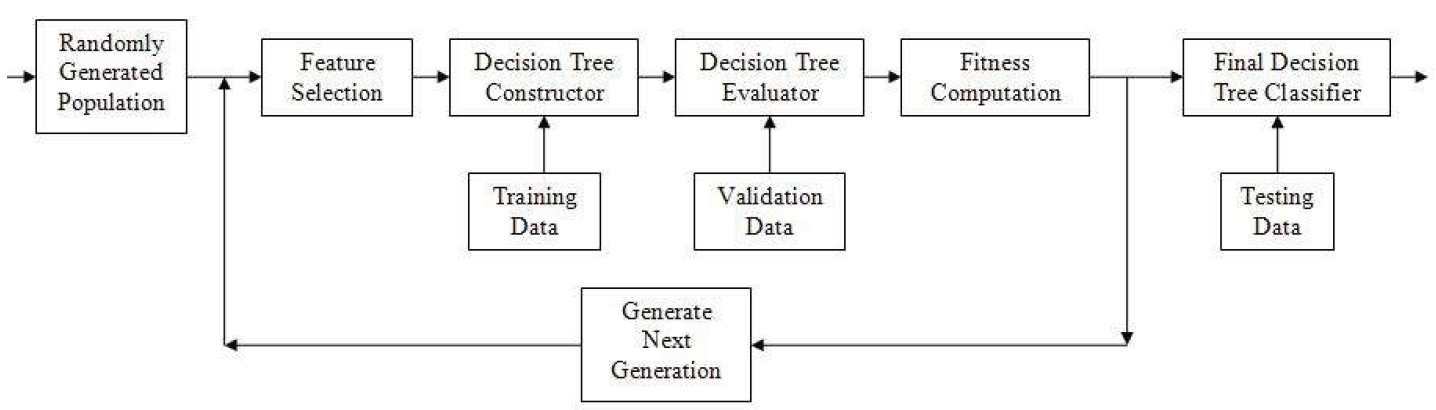
\includegraphics[scale=0.25]{dfd.png}
\caption{The data flow in DT/GA Hybrid Classifier.}
\end{figure}



\section{Object-Oriented Design and Results}






The results of the GA-based optimization scheme is shown in the Figure 2.
\begin{figure}[h!]
  
  \centering
    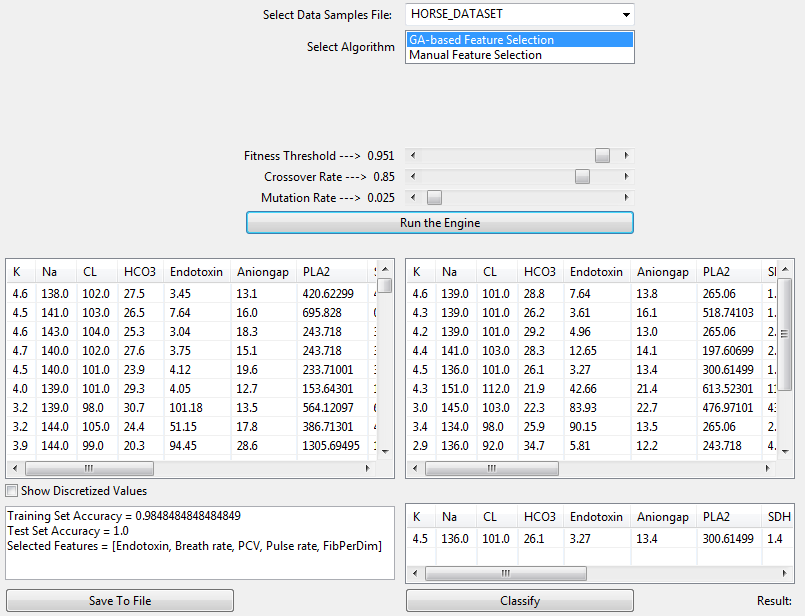
\includegraphics[scale=0.4]{ga_algo_stats.png}
\caption{DT built with GA based feature selection.}
\end{figure}

The results obtained with manual feature selection is shown in Figure 3.
\begin{figure}[h!]
  
  \centering
    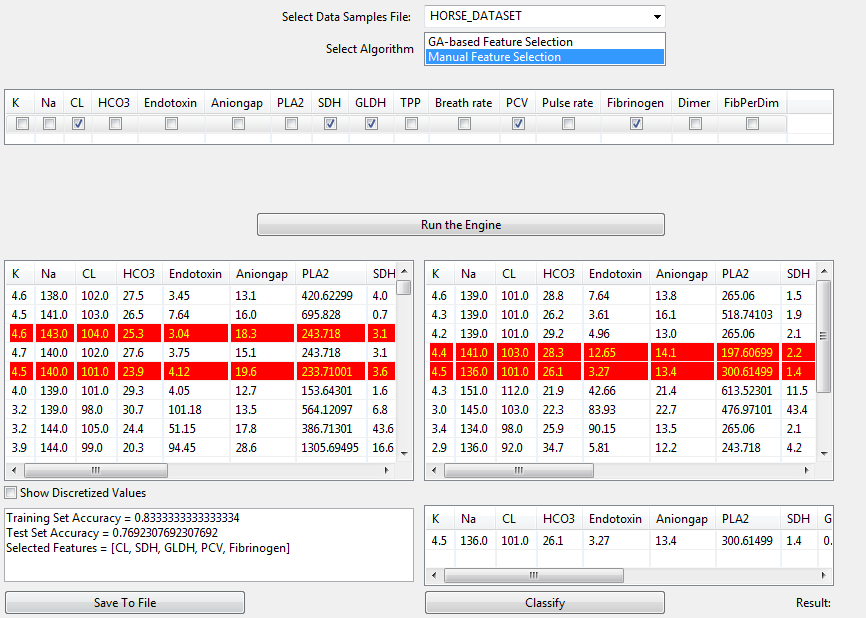
\includegraphics[scale=0.3]{manual_sel_stats.png}
\caption{DT built with manual feature selection.}
\end{figure}
\section{Conclusion}
The genetic algorithm and decision tree hybrid was able to
outperform the decision tree algorithm which was based on manual feature selection.
We believe that this improvement is due to the fact that the
hybrid approach is able to focus on relevant features and
eliminate unnecessary or distracting features. This initial filtering
is able to improve the classification abilities of the decision tree.
The algorithm does take longer to execute than the standard
decision tree; however, its non-deterministic process is able to
make better decision trees. The training process needs only to be
done once. The classification process takes the same amount of
time for the hybrid and non-hybrid systems.

\section{Future Work}
The hybrid GA /decision tree algorithm needs to be tested
further to realize its true potential. Clearly more work needs to be done. 
The test results show that the Decision Trees constructed using the Genetic algorithm-based feature selector, were more efficient and accurate in classifying the data than the Decision Trees constructed by selecting features manually. A forest of decision trees will be
constructed from the combination of four final decision trees,
each for one major attack category. The final decision will be
made through a voting algorithm. We will then compare the
overall classification ability of the hybrid algorithm with other
machine learning algorithms in the literature.

Some other future enhancements could include one of the following:
\begin{enumerate}
\item{The application could be made more responsive by using Threads and Parallel/Cloud Computing}
\item{The Decision Tree Classifier of this application could be optimized using Neural Networks which are more efficient than Decision Trees.}
\item{An interesting extension to be explored is the possibility of
additional feedback from ID3 concerning the evaluation of a
feature set. Currently only classification accuracy is returned.
However, there is potentially exploitable information with
respect to which features were actually used to build the
decision tree and their relative positions in the tree.}

\end{enumerate}


\begin{thebibliography}{1}

\bibitem{textbook}
Hua;Kien A., Wu;Annie S.; Chen;Bing, Stein;Gary
\emph{Decision Tree Classifier For Network Intrusion Detection
With GA-based Feature Selection}

\bibitem{paper}
Jing Xu, Ming Zhao,José Fortes, Robert Carpenter,
Mazin Yousif. \emph{Autonomic resource management in virtualized data centers using
fuzzy logic-based approaches} Cluster Comput (2008) 11: 213–227
DOI 10.1007/s10586-008-0060-0
\bibitem{paper}
T. Wood et al., \emph{Sandpiper.Black-box and gray-box resource management for virtual machines}, Computer Network (2009), doi:10.1016/j.comnet.2009.04.014
\end{thebibliography}

\end{document}


